\section{Method}
% CONTENT GOAL: Describe the frozen product pipeline and the Candidate v3.1 evidence-selection fix at code-verifiable granularity.
% QUESTIONS FOR AUTHORS: Which data structures and interfaces require formal notation? Which implementation details belong in the appendix?
% VERIFIED FACT: Retrieval uses text, vector, assertion, graph, and subject-attachment channels before source-aware fusion and query-aware evidence selection.
% VERIFIED FACT: Benchmark Gold never enters the product retrieval path.
% EVIDENCE: docs/omni-context-paper-evidence-v1/architecture/final-product-fix.md
% EVIDENCE: docs/omni-context-paper-evidence-v1/architecture/module-to-code-map.csv
% ALLOWED: Describe the frozen implementation and its verified internal preflight behavior.
% FORBIDDEN: Claim that the fix universally improves retrieval.

\begin{figure*}[t]
  \centering
  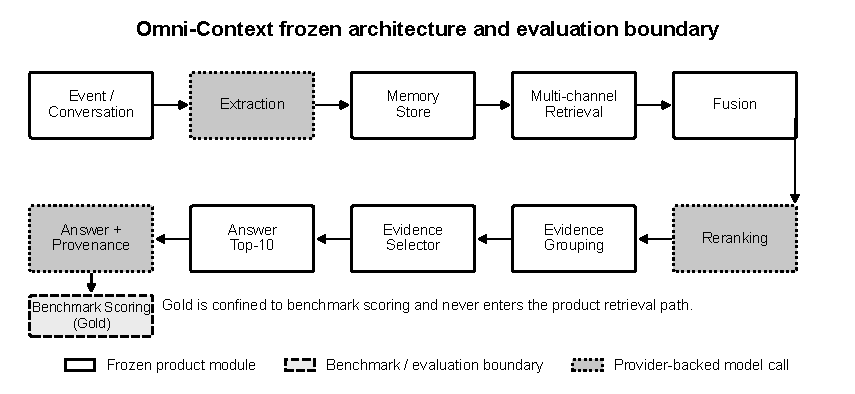
\includegraphics[width=\textwidth]{../figures/architecture.pdf}
  \caption{Frozen product architecture and evaluation boundary. Product modules, benchmark boundaries, and provider-backed calls use distinct line/fill styles.}
  \label{fig:architecture}
\end{figure*}

\begin{figure*}[t]
  \centering
  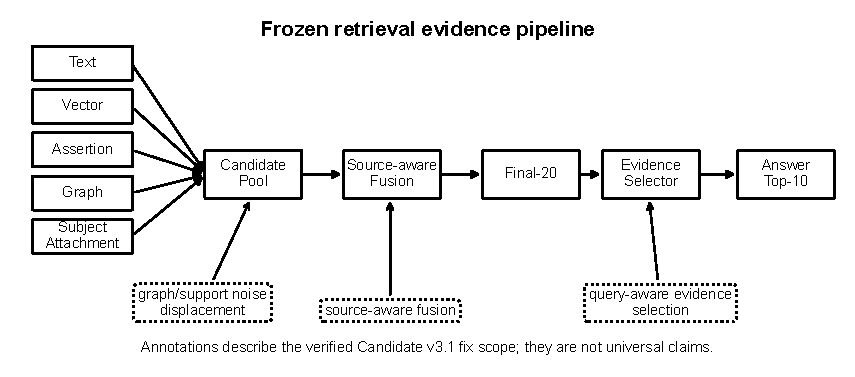
\includegraphics[width=\textwidth]{../figures/retrieval-pipeline.pdf}
  \caption{Evidence retrieval pipeline and the bounded scope of the final Candidate v3.1 fix.}
  \label{fig:retrieval-pipeline}
\end{figure*}

\TODO{Author prose required.}
